\documentclass[runningheads]{llncs}
\usepackage{amsmath,amssymb}
\usepackage{graphicx}
\usepackage{latexsym,graphicx}
\usepackage{xcolor}
\usepackage{url}
\usepackage{algorithm}
\usepackage{algorithmic}
\usepackage{verbatim}

\usepackage{url}
\usepackage{mathrsfs}

\usepackage{tikz}
\usepackage{calc}
\usetikzlibrary{arrows,automata,positioning,shapes}
\tikzstyle{rstate}=[state,ellipse]
\tikzset{>={latex}}



\spnewtheorem{observation}[definition]{Observation}{\bfseries}{\itshape}


\renewcommand{\alph}{{\mathbf{alph}}}
\newcommand{\ord}{{\mathbf{ord}}}
\newcommand{\nat}{\bbbn}
\newcommand{\bigo}{{\mathcal{O}}}
\newcommand{\ra}{\rightarrow}
\newcommand{\pre}{\leq_p}
\newcommand{\suf}{\leq_s}
\newcommand{\id}{\mathbf{id}}

\newcommand{\per}{{per}}
\newcommand{\lper}{{lper}}
\newcommand{\minper}{{\bf minper}}
\newcommand{\ident}{\bf{1}}
\def\ur{\uparrow}
\def\xor{{\bf\ xor\ }}
\renewcommand{\lg}{\log}
\newcommand{\eps}{\epsilon}
\newcommand{\LCP}{{\mathit{LCP}}}
\newcommand{\RMQ}{{\mathit{RMQ}}}
\newcommand{\RmQ}{{\mathit{RmQ}}}
\newcommand{\posRMQ}{{\mathit{posRMQ}}}
\newcommand{\posRmQ}{{\mathit{posRmQ}}}
\newcommand{\LCSuf}{{\mathit{LCS}}}
\newcommand{\LPF}{{\mathit{LPrF}}}
\newcommand{\lmp}{{\mathit{LPnF}}}

\newcommand{\PSC}{{\mathit{PSC}}}
\newcommand{\SSC}{{\mathit{SSC}}}
\newcommand{\PSSC}{{\mathit{PSSC}}}

\newcommand{\PD}{{\mathit{PD}}}
\newcommand{\SD}{{\mathit{SD}}}
\newcommand{\PSD}{{\mathit{PSD}}}
\newcommand{\MRE}{{\mathit{MinRightEnd}}}
\newcommand{\MLE}{{\mathit{MaxLeftEnd}}}


\begin{document}

\title{Testing -binomial equivalence\thanks{The results presented in this paper were partly obtained during the Dagstuhl seminar 14111, in March 2014. Dominik D. Freydenberger was supported by the DFG grant FR 3551/1-1. Pawe{\l} Gawrychowski is currently holding a post-doctoral position at Warsaw Center of Mathematics and Computer Science. Juhani Karhum\"aki was supported by Academy of Finland under the grant 257857. Florin Manea was supported by the DFG grant 596676. Wojciech Rytter was supported by the grant NCN2014/13/B/ST6/00770 of the Polish Science Center. }
}
\titlerunning{Testing -binomial equivalence}

\author{Dominik D. Freydenberger\inst{1} \and Pawe{\l} Gawrychowski\inst{2,3} \and Juhani Karhum\"aki\inst{4} \and \mbox{Florin Manea\inst{5}} \and Wojciech Rytter\inst{2}}
\authorrunning{Freydenberger et al.}

\institute{
Institute for Computer Science, University of Bayreuth, Germany\\ \email{ddfy@ddfy.de}\\
\and Institute of Informatics, University of Warsaw, Poland\\ \email{gawry,rytter@mimuw.edu.pl}\\
\and Institute of Computer Science, University of Wroc{\l}aw, Poland\\
\and Department of Mathematics and Statistics, University of Turku, Finland\\ \email{karhumak@utu.fi}\\
\and Department of Computer Science, Kiel University, Germany\\ \email{flm@informatik.uni-kiel.de}
}

\maketitle

\begin{abstract}
Two words  and  are said to be -binomial equivalent if every non-empty word  of length at most  over the alphabet of  and  appears as a scattered factor of  exactly as many times as it appears as a scattered factor of . We give two different polynomial-time algorithms testing the -binomial equivalence of two words. The first one is deterministic (but the degree of the
corresponding polynomial is too high) while the second one is randomised (but more direct and efficient). \end{abstract}

\section{Introduction}
An {\it alphabet} is a finite and nonempty set of symbols (also called letters). Any finite sequence of symbols from an alphabet  is called a {\it word} over . The set of all words over  is denoted by  and the {\em empty word} is denoted by ; also  is the set of non-empty words over ,  is the set of all words over  of length exactly , while  is the set of all words over  of length at most . Given a word  over an alphabet , we denote by  its length; for some  we denote the -th letter of  by . We also denote the factor that starts with the -th letter and ends with the -th letter in  by . For  we denote by  the number of distinct occurrences of  as a factor of . 

A \emph{scattered factor} of  is a word  for some  such that  for all . The \emph{binomial coefficient} of  and , denoted , equals the number of occurrences of  as a scattered factor of . Clearly, for  we have , while for  with  it is not necessary that . 
For example, if  and  we have , as ; clearly, .

For more details regarding these binomial coefficients see Chapter 6, by Sakarovitch and Simon, from the handbook \cite{Loth97}.

A well known equivalence relation between words is that of abelian equivalence. Two words  are said to be \emph{abelian equivalent} if for all  we have  ; equivalently,  and  are abelian equivalent if they have the same Parikh vector, thus being permutations of each other. This relation was extended in~\cite{KSZ13} (see also \cite{HuKaSaSa11}), where the \emph{-abelian equivalence} relation was defined. Two words  are said to be \emph{-abelian equivalent} if for all  we have . Obviously, the -abelian equivalence relation is the same as the abelian equivalence.

As , another way to generalise the abelian equivalence relation is to define the \emph{-binomial equivalence} (see the conference paper \cite{RigoWORDS}, as well as its journal version \cite{rigo1}). Two words  are said to be \emph{-binomial equivalent} if for all  we have ; if  and  are -binomial equivalent, we write . Again, it is easy to see that the -binomial equivalence is the same as the abelian equivalence. Combinatorial properties of the -binomial equivalence relation are studied in \cite{RigoWORDS,rigo1,rigo2}. 

Recently, in \cite{EhMaMeNo14,EMMN15} a series of algorithmic results regarding the -abelian equivalence were shown. As a basic result, it was shown that one can test whether two words are -abelian equivalent in linear time. Therefore, it seems natural to us to study a similar problem in the context of -binomial equivalence. That is, we are interested in the following problem.

\begin{problem}\label{k-binom-equiv}
Given , with , and , decide whether .
\end{problem}

Our main result shows that Problem \ref{k-binom-equiv} can be solved in polynomial time. The proof of this result uses a series of known results from the theory of finite automata, which does not exploit in any way the properties of -binomial equivalence. Moreover, the degree of the polynomial characterising the time complexity of this algorithm is rather high, so we do not give it explicitly. Instead, we also show a simpler and much more direct Monte-Carlo algorithm solving the same problem. Our solutions assume a basic understanding of formal languages and automata theory; for more details, see \cite{roz:han} and \cite{Sak09}.

The main motivation of studying the algorithmic properties of the -binomial equivalence relation is of fundamental nature: we have a new relation on words and we are, naturally, interested in how we can effectively test whether two words are equivalent with respect to this relation. Our results are also motivated by the work done in avoidability of -binomial repetitions (e.g., squares and cubes in \cite{rigo2}). Constructing infinite words avoiding consecutive occurrences of factors from the same equivalence class with respect to the -binomial equivalence often requires extensive computer simulations, whose basic operation is testing whether two consecutive factors are equivalent. As the words one constructs in such simulations are getting longer and longer, so do their factors whose equivalence one needs to test; consequently, efficient algorithms for testing the equivalence of words are required.

Before moving to the main sections of this paper, we just point out that the complexity results we show here hold in the unit-cost RAM with logarithmic size memory word. In this model (which is generally used in the analysis of algorithms) we assume that, if the size of the input is  (e.g., we are given a word of length ), each memory cell can store  bits, or, in other words, that {\em the machine word size} is . The instructions are executed one after another, with no concurrent operations. The model contains common instructions: arithmetic (add, subtract, multiply, divide, remainder, shifts and bitwise operations, equality testing, etc.), data movement (indirect addressing, load the content of a memory cell, store a number in a memory cell, copy the content of a memory cell to another), and control (conditional and unconditional branch, subroutine call and return). Each such instruction takes a constant amount of time.  This model allows measuring the number of instructions executed in an algorithm, making abstraction of the time spent to execute each of the basic instructions.

\section{A polynomial deterministic algorithm}

The first step we take towards solving Problem \ref{k-binom-equiv} is to construct, for a word , a non-deterministic finite automaton  that accepts exactly the scattered factors of length at most  of  and, moreover, has exactly  paths labelled with the scattered factor  of . 

Let us assume that ; then  has  states; these states are 
 
The initial state of the automaton is , while every state  with  and  is final. The state  is an error state; this state and the initial state are the only states that are not final.

We define the transition function  for all  and all  by

See Figure \ref{fig1} for an illustration. An immediate consequence of this definition is that   holds for all .
\begin{figure}
\begin{center}
  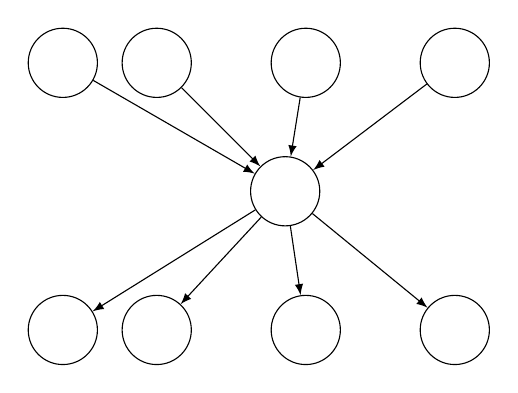
\begin{tikzpicture}[]
    \node[rstate] (top1) {};
    \node[rstate, right=0.3 of top1] (top2) {};
    \node[rstate, right=of top2] (top3) {};
    \node[rstate, right=of top3] (top4) {};

    \node[rstate, below right=of top2] (boss) {};

    \node[rstate, below=2.5 of top1] (bot1) {};
    \node[rstate, right=0.3 of bot1] (bot2) {};
    \node[rstate, right=of bot2] (bot3) {};
    \node[rstate, right=of bot3] (bot4) {};
    \path (top2) -- node {} (top3);
    \path (top3) -- node {} (top4);
    \path (bot2) -- node {} (bot3);
    \path (bot3) -- node {} (bot4);
	\path[->]
		(top1) edge node[left=1.5em] {} (boss)
		(top2) edge node[right] {} (boss)
		(top3) edge node[right] {} (boss)
		(top4) edge node[right=1em] {} (boss)
		(boss) edge node[left=1em] {} (bot1)
		(boss) edge node[right] {} (bot2)
		(boss) edge node[right] {} (bot3)
		(boss) edge node[right=1em] {} (bot4);
  \end{tikzpicture}
\end{center}
\caption{The definition of the transition function: all the transitions leaving  and leading to a non-error state, as well as all transitions going to . We have , with  and .
}
\label{fig1}
\end{figure}

It is not hard to see that  accepts exactly the words  with  and . Indeed, to accept such a word the automaton starts in the state , and then goes through the states 
 
as  it is clear that , so the state reached by the automaton is an accepting one. For the reverse implication, assume that the word  is accepted by  on the path formed by the states 
 

By the definition of  we immediately get that  for all ; also, . Thus,  . Moreover, each transition ending in  is labelled with , so  is a scattered factor of . 

Finally, the argument above shows that there is a bijective correspondence between the sequences of indices defining the scattered factors of length at most  of  and the paths of . In conclusion,  accepts the set of scattered factors of length at most  of  and, moreover, has exactly as many paths labelled with the scattered factor  of  as the total number of occurrences of  as a scattered factor of  (i.e., ). 

Before coming back to the solution Problem \ref{k-binom-equiv}, we recall that two non-deterministic finite automata are said to be \emph{path-equivalent} if for each word  the number of distinct accepting paths labelled with  of  equals the number of distinct accepting paths labelled with  of , or both are infinite. 

In our problem, we were given  and  and wanted to test whether . By the above, it is enough to construct  and  and test whether  and  are path-equivalent. The latter property is decidable (see \cite{siamNFA,Sak09} and the references within for a discussion on this problem and its complexity).

In the following, we show that this algorithm runs in polynomial time in our model of computation. The construction of the two automata  and  takes  time. Moreover, as none of  and  has transitions labelled with , it follows from \cite{siamNFA} that there is an algorithm deciding the path-equivalence of  and  that runs in polynomial time with respect to the size of these automata (so, essentially, with respect to ). Note that the algorithm presented in \cite{siamNFA} is only shown to run in polynomial time in a computational model where it is assumed that the arithmetic operations between any (no matter how big) rational numbers can be done in constant time. To show that the algorithm still runs in polynomial time in our model of computation, we need to go further into details. 

Basically, the algorithm of \cite{siamNFA} applied to the two automata we constructed either decides that  and  identifies the lexicographically first word  such that  has a different number of accepting paths labelled with  than . To do this, the algorithm explores the set of words from  in lexicographical order; it maintains a list of words  and for each  the array  storing the number of accepting paths in  and  (that is, an array storing for each final state of the two automata, how many paths labelled with  connect the initial state of the respective automata to that final state). If the list  contains at some moment the words  and the new considered word is , the algorithm checks if the array  is linearly independent from . If yes,  is added to  and the algorithm further tries all words  with . If no, the algor
 ithm stops trying any other word that has  as a prefix. In \cite{siamNFA} it is shown that only a polynomial number of words should be tried in this process, since  may contain up to  words (as many words as the number of final states of the two automata). In our particular case, it is clear that all words that are longer than  are not accepted by any of our automata (i.e., the array  of some  longer than  contains only s); so, essentially, our algorithm will only try words of length at most . Each such word  that is accepted by one of our automata is accepted on at most  paths, where  is the length of , in total. So, its array  can be stored in at most  memory words (that is,  memory words for each final state, or, in other words,  memory words for each component of the array). At each step of the algorithm, we test whether the newly considered  produces an array  linearly independent from
  the arrays  with ; since all these arrays contain only words that can be stored on  memory words, this test can be done in polynomial time. Indeed, if we use either  a Gaussian elimination method or a modular method, such a test can be implemented in polynomial time (see, e.g., \cite{mulders} and the references within, as well as \cite{Gathen}). Finally, the algorithm just checks whether there exists a word  in  which is accepted on a different number of paths in  than in . Again, this clearly takes polynomial time. 

This concludes our analysis. We do not go into details and compute the exact complexity of the algorithm described above: we just state that it runs in polynomial time. While the preprocessing phase in which  and  are constructed is rather simple, computing the complexity of the algorithm from \cite{siamNFA} requires really going into the implementation details of each step (for instance, testing the linear independency of the arrays), and this is not our purpose. We just note that the exponent of  in the complexity of this algorithm is at least~ (in other words, the algorithm is at least cubic in ). The main result of our paper is, thus, the following theorem. 
\begin{theorem}Problem \ref{k-binom-equiv} can be solved in polynomial time.
\end{theorem}

Although based on a rather simple idea (the construction of the two automata), the algorithm presented in this section has a drawback: the main part of the computation is hidden in the algorithm checking the path equivalence of these two automata. Accordingly, in the following section we present a direct and more efficient randomised algorithm testing the -binomial equivalence of two words.

\section{A Monte-Carlo algorithm}

We begin with a series of prerequisites. The first one is a folklore result; although it is really well known, 
we give a short sketch of the proof for completeness.
\begin{lemma}\label{prime}
We can generate a number  using  operations on -bit numbers, so that  is a random -bit prime with probability at least .
\end{lemma}

\begin{proof}
We recall that, given a -bit number , one iteration of the Rabin-Miller primality test~\cite{RM} performs  operations on -bit numbers, always returns yes if  is prime, and otherwise returns no with probability at least . We choose a random odd -bit number  and execute one iteration of the Rabin-Miller test. If the test succeeds, we return , and otherwise repeat. By Theorem 2 of~\cite{Pomerance}, the procedure returns a composite  with probability less than . However, we need to modify it so that the total number of operations is always .
To this end, we simply terminate after having tried  random -bit numbers.
By the prime number theorem, the probability of a random odd -bit number being prime is . Hence if we generate  such random numbers, the probability of all of them being composite is at most  for  large enough. Therefore, the total error probability is less than  for  large enough. (For smaller , we can use a naive method.) The total number of operations is now always .
\qed
\end{proof}

The second auxiliary result is a particular case of the Schwartz-Zippel lemma. For a prime number , let  denote the finite field on  elements consisting of the integers modulo . It is well known that a non-zero polynomial  of degree  has at most  distinct roots in . Thus, the following trivially holds:
\begin{lemma}\label{SZ}
Let  be a non-zero polynomial of degree  in . Then, the probability that a randomly chosen  is a root of  is at most :
 
\end{lemma}

We now continue with the main part of this section.

For  let  be the number which binary representation is . We define the crucial polynomial:

\begin{example}

\end{example}
Clearly the powers of the variable  encode uniquely the scattered factors of the word , consequently:
\begin{observation}
 if and only if  in .
\end{observation}

By definition, for any word  with , the degree of  is , so we cannot afford (time-wise) to construct it explicitly for any of the words  and , as enumerating the coefficients of such a polynomial would take exponential time. So, what we should see now is how to compute efficiently  in ; this is solved in the next lemma, where we show how  is computed in time  for a word  of length .
In the end we will choose  such that . Consequently, we assume that
operations on numbers in  take  time, because in our model two numbers consisting of
 bits can be added, subtracted, multiplied, and divided in  time.
The bottleneck is that we cannot construct  explicitly, so we need to go around this in order to compute .
\begin{lemma}
For a word  of length , the value  in  can be computed in  time.
\end{lemma}

\begin{proof}
We use an auxiliary polynomial. Let 
In other words  , where  is the number of
scattered occurrences of the word of length  corresponding to the binary expansion of  in the whole word .
For example if  and ,
then , because  and there are four scattered occurrences of  in , i.e., .
It is enough to compute polynomials  since

The additional factor  is needed
since two different words  can start with different number of zeros,
so it can be the case that  despite the fact that, actually, .

We use dynamic programming to compute all , where , , and  is the suffix of  starting at
the -th character. We denote by  the value . Every such  will be computed just once and in time  if we precompute all the numbers  for  in  time.

Then, we just have to compute , which can be done in  time. Hence the claimed overall complexity will follow. 

First, we claim that the following recurrence holds:



This is because of the following reasoning. We write every  as a polynomial in . Then, if the recurrence holds, it can be seen easily that
 is a sum, over all choices of , of monomials of the following form:
 
But this is the same as summing monomials of the form:

Further,  is really the number from  whose binary encoding is the word . 
Therefore, the coefficient of  in  is exactly the number of ways we can choose a scattered factor  of  such that  is the binary encoding of ; in other words, this coefficient equals the number of scattered occurrences of the binary word corresponding to  in .

Consequently, we get that , as claimed. The conclusion of the lemma follows easily.
\qed \end{proof}

We conclude this section by putting together all the preliminary results we have shown, to obtain the final Monte-Carlo algorithm solving Problem \ref{k-binom-equiv}.



\vskip 0.2cm  \begin{small}
    \begin{center}
    \fbox{\vspace*{0.2cm}
    \begin{minipage}{7.1cm}
    \vspace*{0.3cm} \noindent
     \hspace*{0.2cm} {\bf Randomised Algorithm}
     \vskip .2cm
\hspace*{0.2cm} let  be a random -bit prime
\vskip .2cm
\hspace*{0.2cm}
choose random 
\vskip .2cm
\hspace*{0.2cm} compute  and  in 
\vskip .2cm
\hspace*{0.2cm} 
\vskip .2cm
 \hspace*{0.2cm} {\bf return }
 YES if , NO otherwise
 \vspace*{0.2cm}
  \end{minipage}
  }
  \end{center}
  \end{small}
  
The overall time complexity is clearly polynomial both in  and in ; as , we conclude that this algorithm runs in polynomial time. More precisely, generating a prime number requires  operations, where . Then, we use  operations to fill the table. Therefore, the total time complexity is . By considering the case  and  separately, we conclude that the total time complexity is .

Now, if  then  for all , so the algorithm will always return YES.
Otherwise, there are three ways it could err. First, we could have generated a composite .
This happens with probability at most .
Second, it might happen that  is non-zero in the integers, but vanishes in the integers modulo .
By definition, the coefficients of  are bounded by , so if the polynomial is non-zero in the integers, yet vanishes modulo ,  must be a prime divisor of a fixed number bounded by . It is well known that the number of distinct prime divisors of , denoted , satisfies . Because there are  primes in the interval , for  large enough this happens with probability at most .
Third, our choice of  might have been unfortunate. By the Schwartz-Zippel lemma,
this happens with probability at most .
By the union bound, for large enough , the total error probability is, consequently, less than  as required.

\begin{theorem}
Problem \ref{k-binom-equiv}, for input words of length , can be solved by a Monte-Carlo algorithm with running time . The algorithm always returns a positive answer when the input words  and  are -binomial equivalent, and returns a negative answer when  and  are not -binomial equivalent with probability at least .
\end{theorem}

\section{Conclusion}
In this paper we considered the problem of deciding whether two given words  and  are -binomial equivalent. We gave two polynomial algorithms solving this problem. The first one was deterministic, and was heavily relying on a known result showing that deciding whether two non-deterministic finite automata are path-equivalent can be done in linear time. The second one was a direct algorithm, its running time was linear in the length of the input words, but it was no longer deterministic. 

The main consequence of our result is that also finding all the factors of a long word which are -binomial equivalent to a shorter one can be done in polynomial time; in other words, the problem of pattern matching under -binomial equivalence can be solved in polynomial time. Indeed, one can check (using the algorithms presented in this paper) for all factors of the text whether they are -binomial equivalent to the pattern and return those for which this property holds. The next theorem follows.
\begin{theorem}
Given two words  and  and a number , we can find all the factors of  that are -binomial equivalent to  in polynomial time.
\end{theorem}

The main open problems remaining from this work are to find simpler and more efficient algorithms solving Problem \ref{k-binom-equiv} as well as a pattern matching under -binomial equivalence solution that does not use testing -binomial equivalence as a subroutine. 


\section*{Acknowledgements}
We thank Manfred Kufleitner and Eric Rowland for participating in the discussions on this problem during the Dagstuhl seminar 14111, that finally lead to the work presented here.

\bibliographystyle{splncs03}
\bibliography{k-binomial}

\end{document}
